\pagebreak
\section{Magnetometer Calibration} \label{app:magnetoCalibration}
\textbf{Name: Group 510}\\
\textbf{Date: 26/11 - 2015}

\subsection{Purpose}
The purpose of this test is to ensure the fact that the magnetometer is calibrated so that it can tell a correct position relative to the Earth's magnetic field when placed on the vehicle.

\subsection{Theory}
The HMC5883L chip is a magnetometer which uses the Earth's magnetic field as a reference. When using it for the first time it is necessary to calibrate it so that disturbances in the close field of the sensor are accounted for in later measurements.\\
%
In this project the disturbances can be caused by all the metallic pieces on the vehicle, from the metal plate to the motor and to the wires. Thus, the calibration has to be performed with the all these components and the sensor placed on the vehicle at a fixed place and orientation. It is chosen to place it, so that its X axis points towards the front of the vehicle and the Z axis is pointed upwards. The chosen configuration shall not be changed after calibration.\\
%
As stated in \secref{sec:magnetoSensor}, the magnetometer that is used gives out three space coordinates of the Earth's magnitude field relative to its own coordinate system. One good to test to see if the sensor is operational in its environment is to turn it all around itself while retrieving the data it gives. When properly calibrated and isolated from any new disturbance, the 3D scatter plot of all the measured points should give a sphere that has its center in the origin (coordinates (0,0,0)) of the plot. This means that the measured coordinates vary smoothly accordingly with the rotation of the sensor in space. Otherwise, the sphere could be distorted into an ellipsoid and displaced from the center and the sensor would have to be recalibrated correctly in a magnetic-still environment.\\
%
The calibration itself performed in this test does not change the intrinsic sensor configuration but rather applies a transformation to the coordinates sent to the Arduino board. This transformation, as seen in \eqref{eq:calibrationTransformation} is actually computed in the runtime by the microcontroller, each time a set of coordinate is received :
\begin{flalign}
  \begin{pmatrix} 
    x_{cal} \\
    y_{cal} \\
    z_{cal} 
  \end{pmatrix}
  =
  \begin{pmatrix} 
    m_{1,1} & m_{1,2} & m_{1,3} \\
    m_{2,1} & m_{2,2} & m_{2,3} \\
    m_{3,1} & m_{3,2} & m_{3,3} 
  \end{pmatrix}
  \cdot
  \begin{pmatrix} 
    x_{measured} \\
    y_{measured} \\ 
    z_{measured} 
  \end{pmatrix} 
  + 
  \begin{pmatrix} 
    b_x \\ 
    b_y \\ 
    b_z 
  \end{pmatrix}
% \eq{m}{ \cdot  } \unit{^{\circ}}
\label{eq:calibrationTransformation}
\end{flalign}
\todo{Try to put this in the eq environment}





% \begin{figure}[H]
%   \centering
%   %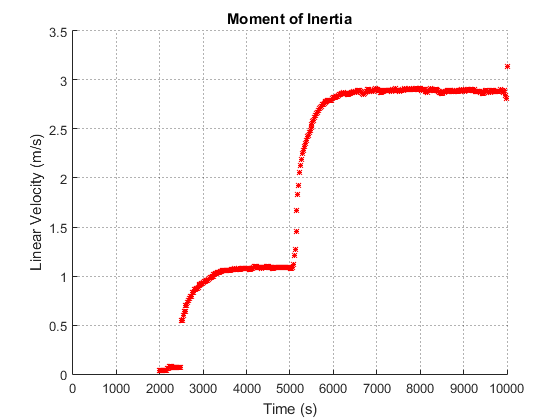
\includegraphics[scale=0.8]{figures/VehicleMomentOfInertiaTest.png}
%   \caption{Vehicle's velocity response to a two-steps input}
%   \label{fig:MomentOfInertiaTestPlot}
% \end{figure}

%% Test setup description %%
\subsection{Setup}
\begin{figure}[H]
  \centering
  %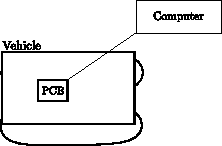
\includegraphics[scale=1.6]{figures/inertiaTestSetupDiagram2.pdf}
  \caption{Setup diagram}
  \label{calibrationSetupDiagram}
\end{figure}

\subsection{List of Equipment}

\begin{table}[H]
\begin{tabular}{|p{10cm}|p{4cm}|}
\hline%------------------------------------------------------------------------------------
  \textbf{Instrument}                     &  \textbf{Type}       \\
\hline%------------------------------------------------------------------------------------
  Computer                                &  HP???    \\
\hline %-----------------------------------------------------------------------------------
\end{tabular}
\end{table}

%% Procedure %%
\subsection{Procedure}

\begin{enumerate}
  \item Step 1
\end{enumerate}

%% Results %%
\subsection{Results} \label{magnetoCalibrationResults}

